%%%%
%% main.tex
%%
%% Copyright 2010 Jeffrey Finkelstein
%%
%% Except where otherwise noted, this work is made available under the terms of
%% the Creative Commons Attribution-ShareAlike 3.0 license,
%% http://creativecommons.org/licenses/by-sa/3.0/.
%%
%% You are free:
%%    * to Share — to copy, distribute and transmit the work
%%    * to Remix — to adapt the work
%% Under the following conditions:
%%    * Attribution — You must attribute the work in the manner specified by
%%    the author or licensor (but not in any way that suggests that they
%%    endorse you or your use of the work).
%%    * Share Alike — If you alter, transform, or build upon this work, you may
%%    distribute the resulting work only under the same, similar or a 
%%    compatible license.
%%    * For any reuse or distribution, you must make clear to others the 
%%    license terms of this work. The best way to do this is with a link to the
%%    web page http://creativecommons.org/licenses/by-sa/3.0/.
%%    * Any of the above conditions can be waived if you get permission from
%%    the copyright holder.
%%    * Nothing in this license impairs or restricts the author's moral rights.
%%%%
\documentclass{article}

% package imports
\usepackage{algorithm2e}
\usepackage{amsmath} % required for piecewise function definition
\usepackage{amsthm} % required for theorems, definitions, lemmas, and styles
\usepackage{amssymb} % required for strict subset symbol (\subsetneq)
\usepackage{chngcntr}
\usepackage{complexity} % required for typesetting complexity classes
\usepackage{cclicenses} % required for adding creative commons license symbols
\usepackage{graphicx} % required for including images
\usepackage{hyperref} % required for hyperlinking references in the article

% define theorem, lemma, and definition environments and corresponding styles
\newtheorem{theorem}{Theorem}[section]
\newtheorem{lemma}{Lemma}[section]
\theoremstyle{definition} 
\newtheorem{definition}{Definition}[section]

% custom shortcut commands
\newcommand{\plain}[1]{\,\text{#1}\,} % plain text inside math environments
\newcommand{\sigmastar}{\Sigma^{*}}
\newcommand{\kr}{\leq^{p}_{ker}} % kernel-reduces
\newcommand{\nkr}{\nleq^{p}_{ker}} % does not kernel-reduce

% create the license
\newcommand{\license}{\begin{tabular}[h]{r l}
    \bysa & \parbox{275pt}{Copyright 2010 Jeffrey Finkelstein. 
      Except where otherwise noted, this work is licensed
      under http://creativecommons.org/licenses/by-sa/3.0/}
\end{tabular}}

% redefine footnote so it has no reference and no number
\long\def\symbolfootnote[#1]#2{\begingroup%
\def\thefootnote{\fnsymbol{footnote}}\footnotetext{#2}\endgroup} 

% change figure numbering so it is per section
\counterwithin{figure}{section}

% define the author, title, and date
\author{Jeffrey Finkelstein} 
\title{Untitled}
\date{\today} 

\begin{document}
\maketitle
\symbolfootnote[0]{\license}
\begin{abstract}
Hello, world!
\end{abstract}
\section{Definitions}

In the following definitions, $x,y\in\sigmastar$.

Let $R_{par}=\{(x, y)|x \plain{and} y \plain{have the same parity}\}$.

Let $R_{bc}=\{(x, y)|x \plain{and} y \plain{have the same number of ones}\}$.

Let $R_{eq}=\{(x, y)|x = y\}$.

Let $R_{eqi}=\{(x, y)|x = y \lor x = \bar{y}\}$.

For any fixed $a\in\sigmastar$, let $R_{a}=\{(x, y)|x = y \lor x \oplus y =
a\}$. ($R_{a}$ is a family of equivalence relations; $R_{a}$ is a different
relation for each $a$.)

Notice the following equivalent definitions, where $n$=$|x|$=$|y|$:
$R_{eq}=\{(x, y)|x \oplus y = 0^n\}$, $R_{eqi}=\{(x, y)|x \oplus y = 0^n \lor x
\oplus y = 1^n\}$, and $R_{a}=\{((a,x),(a,y))|x \oplus y = 0^n \lor x \oplus
y\ = a\}$.

Let $GI=\{(G_1,G_2)|G_1 \plain{and} G_2 \plain{are undirected graphs and} G_1
\plain{is isomorphic to} G_2\}$.

\begin{definition}Let $R,S\subseteq\sigmastar\times\sigmastar$. We say $R$
  \textit{kernel reduces to} $S$ if $\exists f\in\FP:\forall x,y\in\sigmastar
  (x, y)\in R \iff (f(x),f(y))\in S$. We denote this by $R\kr
  S$.\end{definition}

\section{Relationships among equivalence relations}
%% TODO show that all the stated equivalence relations are actually eq. rel.s

\begin{theorem}$R_{eq} \subsetneq R_{bc} \subsetneq R_{par}$\end{theorem}
\begin{proof}
  Let $(x, y)\in R_{eq}$, so $x=y$. Then $x$ has exactly the same number of ones
  as $y$ (and the same number of zeros, and in the same order), so $(x, y) \in
  R_{bc}$. Therefore, $R_{eq} \subset R_{bc}$.
 
  Consider $x=1100$ and $y=0101$. Then $(x, y)\in R_{bc}$ but $(x, y) \notin
  R_{eq}$. Therefore $R_{eq} \neq R_{bc}$.

  Let $(x, y)\in R_{bc}$, so $x$ and $y$ have the same number of ones. Let $k$
  be the number of ones in $x$, and $l$ be the number of ones in $y$. Then
  $l=k$, which implies $l \equiv k (mod 2)$. Therefore $x$ and $y$ have the
  same parity, so $(x, y)\in R_{par}$. Therefore $R_{bc} \subset R_{par}$.

  Consider $x=1000$ and $y=1011$. Then $(x, y)\in R_{par}$ but $(x, y) \notin
  R_{bc}$. Therefore $R_{bc} \neq R_{par}$.
\end{proof}

\begin{theorem}$R_{eq} \subsetneq R_{eqi}$\end{theorem}
\begin{proof}
  Let $(x, y)\in R_{eq}$, so $x=y$. Then $(x, y)$ satisfies the property
  specified in the definition of $R_{eqi}$, specifically that $x=y$, so
  $(x, y) \in R_{eqi}$. Therefore $R_{eq} \subset R_{eqi}$.

  Consider $x=1000$ and $y=0111$. Then $(x, y)\in R_{eqi}$ but $(x, y) \notin
  R_{eq}$. Therefore $R_{eq} \neq R_{eqi}$.
\end{proof}

Figure \ref{fig:containments} exhibits the containments among $R_{eq}$,
$R_{eqi}$, $R_{bc}$, and $R_{par}$. Note that if $a=0^n$, for $n=|x|=|y|$, then
$R_{a}=R_{eq}$ and if $a=1^n$ then $R_{a}=R_{eqi}$.

\begin{figure}
  \begin{center}
    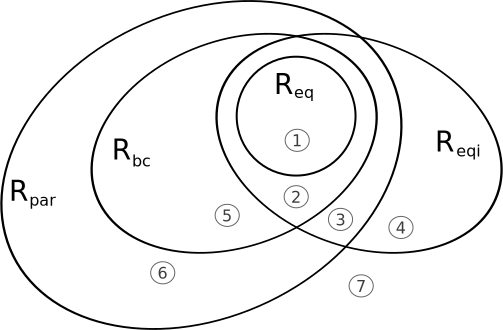
\includegraphics[width=300pt,height=241pt,keepaspectratio=true]
                    {containments.png}
  \end{center}
  \caption{ \label{fig:containments} Containment relationships for equivalence
    relations $R_{eq}$, $R_{eqi}$, $R_{bc}$, and $R_{par}$. The following are
    example elements in the sets at the specified locations: 1. (1100, 1100)
    2. (1010, 0101) 3. (1000, 0111) 4. (10000, 01111) 5. (1000, 0001) 6. (1000,
    1011) 7. (1000, 0000) }
\end{figure}

\section{Results}
\subsection{Reductions among equivalence relation}
%% TODO convert from enumerate blocks to pseudocode blocks
\begin{theorem}$R_{par}\kr R_{bc}$\end{theorem}
\begin{proof}
  Construct $M\in \FP$ on input $w\in\sigmastar$:
  \begin{enumerate}
  \item For $i=1$ to $|w|$:
    \begin{enumerate}
    \item If $w_i = 1$, for $j=i$ to $|w|$:
      \begin{enumerate}
      \item If $w_j = 1$, write a $0$ to $w_i$ and $w_j$
      \item Break
      \end{enumerate}
    \end{enumerate}
  \end{enumerate}
  Notice that this is the machine which finds pairs of ones and writes zeros in
  their place, one pair at a time.

  Suppose $(x, y)\in R_{par}$, so either $x$ and $y$ both have even parity or
  $x$ and $y$ both have odd parity.
  
  If $x$ and $y$ both have even parity, $x$ contains $2k$ ones and $y$ contains
  $2l$ ones, for some $k,l\in\mathbb{N}$. $M(x)$ and $M(y)$ both output the
  string $0^{|x|}$, and since both $M(x)$ and $M(y)$ have a bitcount of zero,
  $(M(x), M(y))\in R_{bc}$.

  If $x$ and $y$ both have odd parity, $x$ contains $2k+1$ ones and $y$
  contains $2l+1$ ones, for some $k,l\in\mathbb{N}$. $M(x)$ and $M(y)$ both
  output a string containing a single one, so both $M(x)$ and $M(y)$ have a
  bitcount of one, $(M(x), M(y))\in R_{bc}$.

  Suppose $(x, y)\notin R_{par}$, so without loss of generality, $x$ has even
  parity and $y$ has odd parity. Then $x$ contains $2k$ ones and $y$ contains
  $2l+1$ ones, for some $k,l\in\mathbb{N}$. Thus $M(x)$ outputs the string
  $0^{|x|}$ and $M(y)$ outputs the string containing a single one. Since the
  bitcount of $M(x)$ is zero and the bitcount of $M(y)$ is one,
  $(M(x), M(y))\notin R_{bc}$.

  Therefore $(x, y)\in R_{par} \iff (M(x), M(y))\in R_{bc}$, so
  $R_{par} \kr R_{bc}$.
\end{proof}

\begin{theorem}$R_{bc}\kr R_{eq}$\end{theorem}
\begin{proof}
  Construct $M\in \FP$ on input $w\in\sigmastar$:
  \begin{enumerate}
  \item Sort the bits of $w$ in increasing order using an efficient (polynomial
    time) sorting algorithm
  \end{enumerate}
  Notice that if $|w|=n$ and $w$ contains $k$ ones, this machine outputs
  the string which can be described by the regular expression $0^{n-k}1^k$.

  Suppose $(x, y)\in R_{bc}$, so $x$ and $y$ have the same number of ones, say
  $k$. Thus $M(x)=M(y)=0^{n-k}1^k$, so $(M(x), M(y))\in R_{eq}$.
  
  Suppose $(x, y)\notin R_{bc}$, so $x$ and $y$ have a different number of
  ones. Suppose $x$ has $k$ ones and $y$ has $l$ ones, for some
  $k,l\in\mathbb{N}$. Assume without loss of generality that $k>l$. Then
  $M(x)=0^{n-k}1^{k}$ and $M(y)=0^{n-l}1^{l}$, so $M(x)\neq M(y)$. Thus
  $(M(x), M(y))\notin R_{eq}$.

  Therefore $(x, y)\in R_{bc} \iff (M(x), M(y))\in R_{eq}$, so $R_{bc}\kr
  R_{eq}$.
\end{proof}

\subsection{Reductions from equivalence relations to graph isomorphism}
\begin{theorem}\label{thm:rpar-gi}$R_{par}\kr GI$\end{theorem}
\begin{proof}
  Construct $M\in \FP$ on input $w\in\sigmastar$:
  \begin{enumerate}
  \item Initialize set of vertices $V_w=\{v_{p}, v_{o}\}$ and set of
    (undirected) edges $E_w=\{\}$.
  \item For $i=1$ to $|w|$:
    \begin{enumerate}
    \item If $w_i=1$ and $(v_{o}, v_{p})\notin E_w$, add undirected edge
      $(v_{o}, v_{p})$ to $E_w$.
    \item Else if $w_i=1$ and $(v_{o}, v_{p})\in E_w$, remove $(v_{o}, v_{p})$
      from $E_w$.
    \end{enumerate}
  \item Output $G_w=(V_w,E_w)$.
  \end{enumerate}

  Suppose $(x, y)\in R_{par}$, so either $x$ and $y$ both have even parity or
  $x$ and $y$ both have odd parity. 

  If $x$ and $y$ both have even parity, $x$ contains $2k$ ones and $y$ contains
  $2l$ ones, for some $k,l\in\mathbb{N}$. Since $2k$ is even, machine $M$ on
  input $x$ adds then removes the edge $(v_o, v_p)$ to and from $E_x$ an equal
  number of times. Similarly for $M$ on input $y$. Therefore $M(x)$ outputs
  $G_x=(V_x, E_x)$, where $V_x=\{v_o, v_p\}$ and $E_x=\{\}$, and $M(y)$ outputs
  $G_y=(V_y, E_y)$, where $V_y=\{v_o, v_p\}$ and $E_y=\{\}$. Then $G_x$ is
  isomorphic to $G_y$ by the identity function, $I:V_x\to V_y$, defined by
  $I(v)=v, \forall v\in V_x$.

  If $x$ and $y$ both have odd parity, $x$ contains $2k+1$ ones and $y$
  contains $2l+1$ ones, for some $k,l\in\mathbb{N}$. Since $2k+1$ is odd,
  machine $M$ on input $x$ adds edge $(v_o, v_p)$ to $E_x$ one more time than
  it removes the edge. Similarly for $M$ on input $y$. Therefore $M(x)$ outputs
  $G_x=(V_x, E_x)$, where $V_x=\{v_o, v_p\}$ and $E_x=\{(v_o, v_p)\}$, and
  $M(y)$ outputs $G_y=(V_y, E_y)$, where $V_y=\{v_o, v_p\}$ and $E_y=\{(v_o,
  v_p)\}$. Then $G_x$ is isomorphic to $G_y$ by the identity function,
  $I:V_x\to V_y$, defined by $I(v)=v, \forall v\in V_x$.

  Suppose $(x, y)\notin R_{par}$, so without loss of generality, $x$ has even
  parity and $y$ has odd parity. Then $x$ contains $2k$ ones and $y$ contains
  $2l+1$ ones, for some $k,l\in\mathbb{N}$. Since $2k$ is even, machine $M$ on
  input $x$ adds then removes the edge $(v_o, v_p)$ to and from $E_x$ an equal
  number of times. Since $2l+1$ is odd, machine $M$ on input $y$ adds edge
  $(v_o, v_p)$ to $E_y$ one more time than it removes the edge. Therefore
  $M(x)$ outputs $G_x=(V_x, E_x)$, where $V_x=\{v_o, v_p\}$ and $E_x=\{\}$, and
  $M(y)$ outputs $G_y=(V_y, E_y)$, where $V_y=\{v_o, v_p\}$ and $E_y=\{(v_o,
  v_p)\}$. Since $(v_o, v_p)\in E_y$ but $(v_o, v_p)\notin E_x$, so no
  bijection exists between $V_x$ and $V_y$ which preserves edges. Therefore,
  $G_x$ is not isomorphic to $G_y$.

  Therefore $(x, y)\in R_{par} \iff (M(x), M(y)) \in GI$, so $R_{par} \kr GI$.
\end{proof}

\begin{theorem}\label{thm:rbc-gi}$R_{bc}\kr GI$\end{theorem}
\begin{proof}
  Construct $M\in \FP$ on input $w \in \sigmastar$:
  \begin{enumerate}
  \item Initialize set of vertices $V_w=\{v_{zero}, v_{one,0}, v_{one,1},
    v_{one,2}\}$ and set of (undirected) edges $E_w=\{(v_{one,0}, v_{one,1}),
    (v_{one,1}, v_{one,2}), (v_{one,2}, v_{one,0})\}$ (so at this point, the
    graph $(V_w, E_w)$ consists of a single vertex connected to no other
    vertices and a triangle consisting of vertices $v_{one,0}$, $v_{one,1}$,
    and $v_{one,2}$).
  \item for $i=1$ to $|w|$:
    \begin{enumerate}
    \item Add $v_i$ to $V_w$.
    \item If $w_i = 1$, add undirected edge $(v_i, v_{one,0})$ to $E_w$.
    \item Else if $w_i = 0$, add undirected edge $(v_i, v_{zero})$ to $E_w$.
    \end{enumerate}
  \item Output $G_w=(V_w, E_w)$.
  \end{enumerate}
  
  Suppose $(x, y)\in R_{bc}$, so $x$ and $y$ have the same number of ones, say
  $k\in\mathbb{N}$. Assume $|x|=|y|=n$, so both $x$ and $y$ have $n-k$
  zeros. Define $E_{w,1}=\{(v_i, v_{one,0})|v_i = 1\}$ and $E_{w,0}=\{(v_i,
  v_{zero})|v_i = 0\}$, so $E_x = E_{x,1}\cup E_{x,0}$ and $E_y = E_{y,1} \cup
  E_{y,0}$ by construction. Define $V_{w,b}=\{v_i|x_i=b\}$, so $V_x=V_{x,1}
  \cup V_{x,0}$ and $V_y=V_{y,1} \cup V_{y,0}$. Note that
  $|V_{x,1}|=|V_{y,1}|=k$ and $|V_{x,0}|=|V_{y,0}|=n-k$. Since
  $|V_{x,1}|=|V_{y,1}|=k$, there exists a bijection between them, call it
  $\phi_1:V_{x,1}\to V_{y,1}$. Similarly, since $|V_{x,0}|=|V_{y,0}|=k$, there
  exists a bijection between them, call it $\phi_0:V_{x,0}\to V_{y,0}$. Define
  $\phi:V_x\to V_y$ by 
  \begin{displaymath}
    \phi(v) = 
    \begin{cases}
      \phi_0(v) & \plain{if} v = v_i \plain{and} x_i = 1, \plain{for some} i\in\{1,\ldots,|x|\}\\
      \phi_1(v) & \plain{if} v = v_i \plain{and} x_i = 0, \plain{for some} i\in\{1,\ldots,|x|\}\\
      v & \plain{if} v \in \{v_{zero}, v_{one,0}, v_{one,1}, v_{one,2}\}
    \end{cases}
  \end{displaymath}
  for all $v\in V_x$. Notice that each $v_i$ ``corresponds'' to a
  single $x_i$, because each $x_i$ can be either a one or a zero,
  exclusively.

  Since the only edges in $E_x$ are the edges $(v_i, v_{one,0})$ when $x_i=1$
  and $(v_i, v_{zero})$ when $x_i=0$, then $(v_i, v_{one,0})\in V_x
  \iff (\phi(v_i), \phi(v_{one,0}))=(\phi_1(v_i), v_{one,0})\in
  V_y$, and $(v_i, v_{zero})\in V_x \iff (\phi(v_i), \phi(v_{zero}))
  = (\phi_0(v_i), v_{zero})\in V_y$. Therefore $\phi$ describes a graph
  isomorphism, so $G_1$ is isomorphic to $G_2$.
  
  Suppose $(x, y)\notin R_{bc}$, so $x$ and $y$ have a different number of
  ones. Let $k$ be the number of ones in $x$, and $l$ be the number of ones in
  $y$, with $k\neq l$. Suppose without loss of generality that $k>l$. Define
  $E_{w,0}$ and $E_{w,1}$ as above. Now $|E_{x,1}|=k$ and $|E_{y,1}|=l$. Since
  $k>l$, $E_{x,1}$ has at least one more edge adjacent to the triangle created
  by the vertices $\{v_{one,0},v_{one,1},v_{one,2}\}$ than does $E_{y,1}$. Thus
  no possible bijection exists between $V_x$ and $V_y$ which preserves all
  edges. Thus $G_x$ is not isomorphic to $G_y$, so $(M(x), M(y))\notin GI$.

  Therefore $(x, y)\in R_{bc} \iff (M(x), M(y))\in GI$, so $R_{bc}\kr GI$.
\end{proof}

\begin{theorem}$R_{eq} \kr GI$\end{theorem}
\begin{proof}The proof is similar as the proofs of Theorems \ref{thm:rpar-gi}
  and \ref{thm:rbc-gi}, but uses a directed graph instead of an undirected
  graph. Since undirected graph isomorphism is polynomial time equivalent to
  directed graph isomorphism, the proof is complete.\end{proof}
\begin{proof}
  Construct machine $M\in\FP$ on input $w\in\sigmastar$:
  \begin{enumerate}
  \item Initialize set of vertices $V_w=\{v_1, v_2, \ldots, v_{|w|}\}$
    and set of directed edges $E_w=\{(v_1, v_2),(v_2,
    v_3),\ldots,(v_{|w|-1}, v_{|w|})\}$.
  \item For $i=1$ to $|w|$:
    \begin{enumerate}
    \item If $w_i=1$, add vertex $v'_i$ to $V_w$ and directed edge $(v_i,
      v'_i)$ to $E_w$.
    \end{enumerate}
  \item Output $G_w=(V_w, E_w)$.
  \end{enumerate}
  This machine constructs a ``spine'' of vertices, with an extra vertex $v'_i$
  and directed edge $(v_i, v'_i)$ adjacent to the spine whenever $w_i$ is a
  one, $\forall i\in\{1,2,\ldots,|w|\}$.

  Suppose $(x, y)\in R_{eq}$, so $x=y$. Then $M(x)$ and $M(y)$ obviously
  produce the same graph, so $(M(x), M(y))\in GI$.
  
  %% TODO is this sufficient proof?

  Suppose $(x, y)\notin R_{eq}$, so $x\neq y$. Suppose $|x|=|y|=n$. Run $M$ on
  input $x$ to yield $G_x=(V_x, E_x)$, and run $M$ on input $y$ to yield
  $G_y=(V_y, E_y)$. Since the graphs are directed, the ``spine'' created by the
  vertices $\{v_1, v_2, \ldots, v_n\}$ and the edges $\{(v_1, v_2), (v_2, v_3),
  \ldots, (v_{n-1}, v_n)\}$ must correspond in both $G_x$ and $G_y$. Let $i$ be
  the index of the first bit at which $x$ and $y$ differ. Suppose without loss
  of generality that $x_i=1$ and $y_i=0$. Then $v'_i\in V_x$ and $(v_i,
  v'_i)\in E_x$, but $v'_i\notin V_y$ so $(v_i, v'_i)\notin E_y$. Since
  vertices along the ``spine'' of the $V_x$ must map to vertices along the
  ``spine'' of $V_y$, and specifically $v_i$ in $V_x$ must map to $v_i$ in
  $V_y$, $(v_i, v'_i)\in E_x$ implies $(v_i, v'_i)\in E_y$. But no such mapping
  can exist, because $(v_i, v'_i)\notin E_y$. Therefore $G_x$ is not isomorphic
  to $G_y$, so $(M(x), M(y))\notin GI$.

  Therefore $(x, y)\in R_{eq} \iff (M(x), M(y))\in GI$, so $R_{eq}\kr GI$.  
\end{proof}

\begin{theorem}$R_{eqi}\kr GI$\end{theorem}
\begin{proof}
  Construct machine $M\in \FP$ on input $w\in\sigmastar$:
  \begin{enumerate}
  \item For $i=1$ to $|w|$:
  \end{enumerate}
\end{proof}
\end{document}
